\newpage

\section{实验与基准测试补充细节}

\subsection{系统与库}
\label{sec:system}

我们在B100 180GB SXM6（1000W）上对速度进行基准测试。
预热5次后，重复基准测试10次，取平均计时。

我们通常使用撰写本文时（2025年3月）各库的最新版本。
具体使用版本：
\begin{itemize}
\item CUDA 13.1
\item \fa 2.8.3
\item Triton 3.6
\item PyTorch 2.10.0
\item CuTe-DSL 4.4.1 
\end{itemize}
对于cuDNN，主论文中我们与cuDNN 9.13和最新版本cuDNN 9.19.1.2进行比较。从9.13和9.14版本起~\citep{cudnn913releasenotes}，我们与cuDNN团队合作，将\faf的部分技术纳入cuDNN，使我们的工作能惠及尽可能多的实践者。

\subsection{确定性非因果后向传播}

为完整起见，我们在图~\ref{fig:bwd-det-ablation-non-causal}中展示了无因果掩码条件下确定性后向内核的性能，与因果掩码情况并排对比。

\begin{figure*}[t]
\centering
 \begin{minipage}{0.48\textwidth}
    \centering
    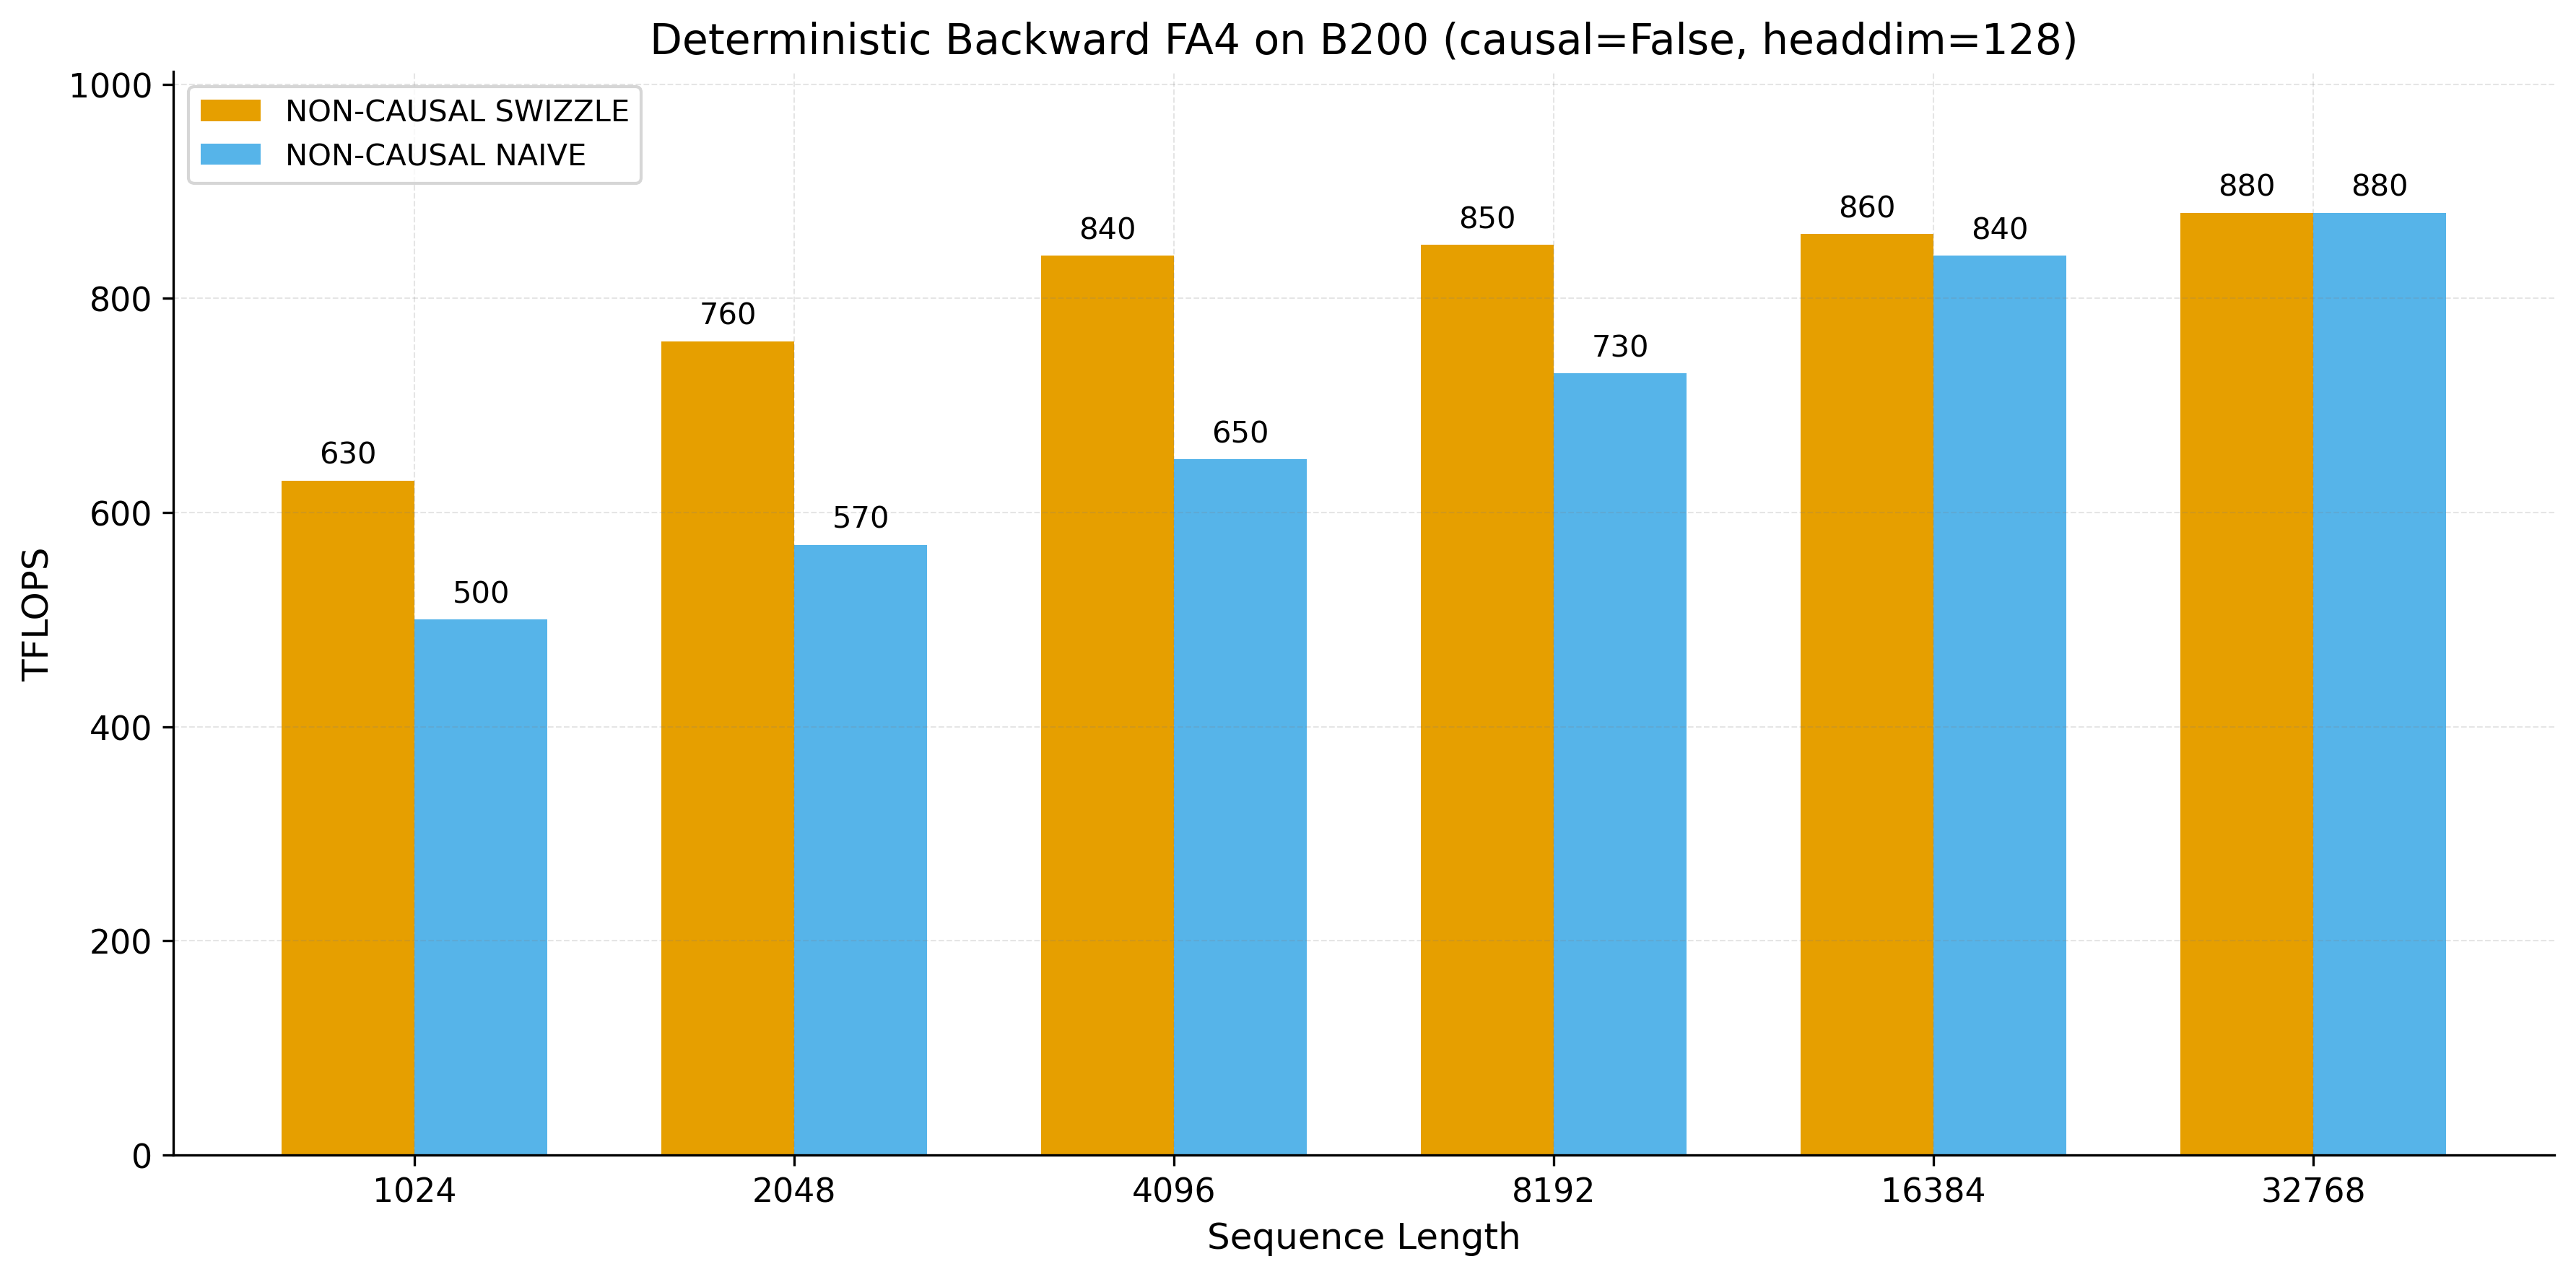
\includegraphics[width=\textwidth]{../Figures/non-causal_bwd_det_FA4.png}
  \end{minipage}
  \hfill
  \begin{minipage}{0.48\textwidth}
    \centering
    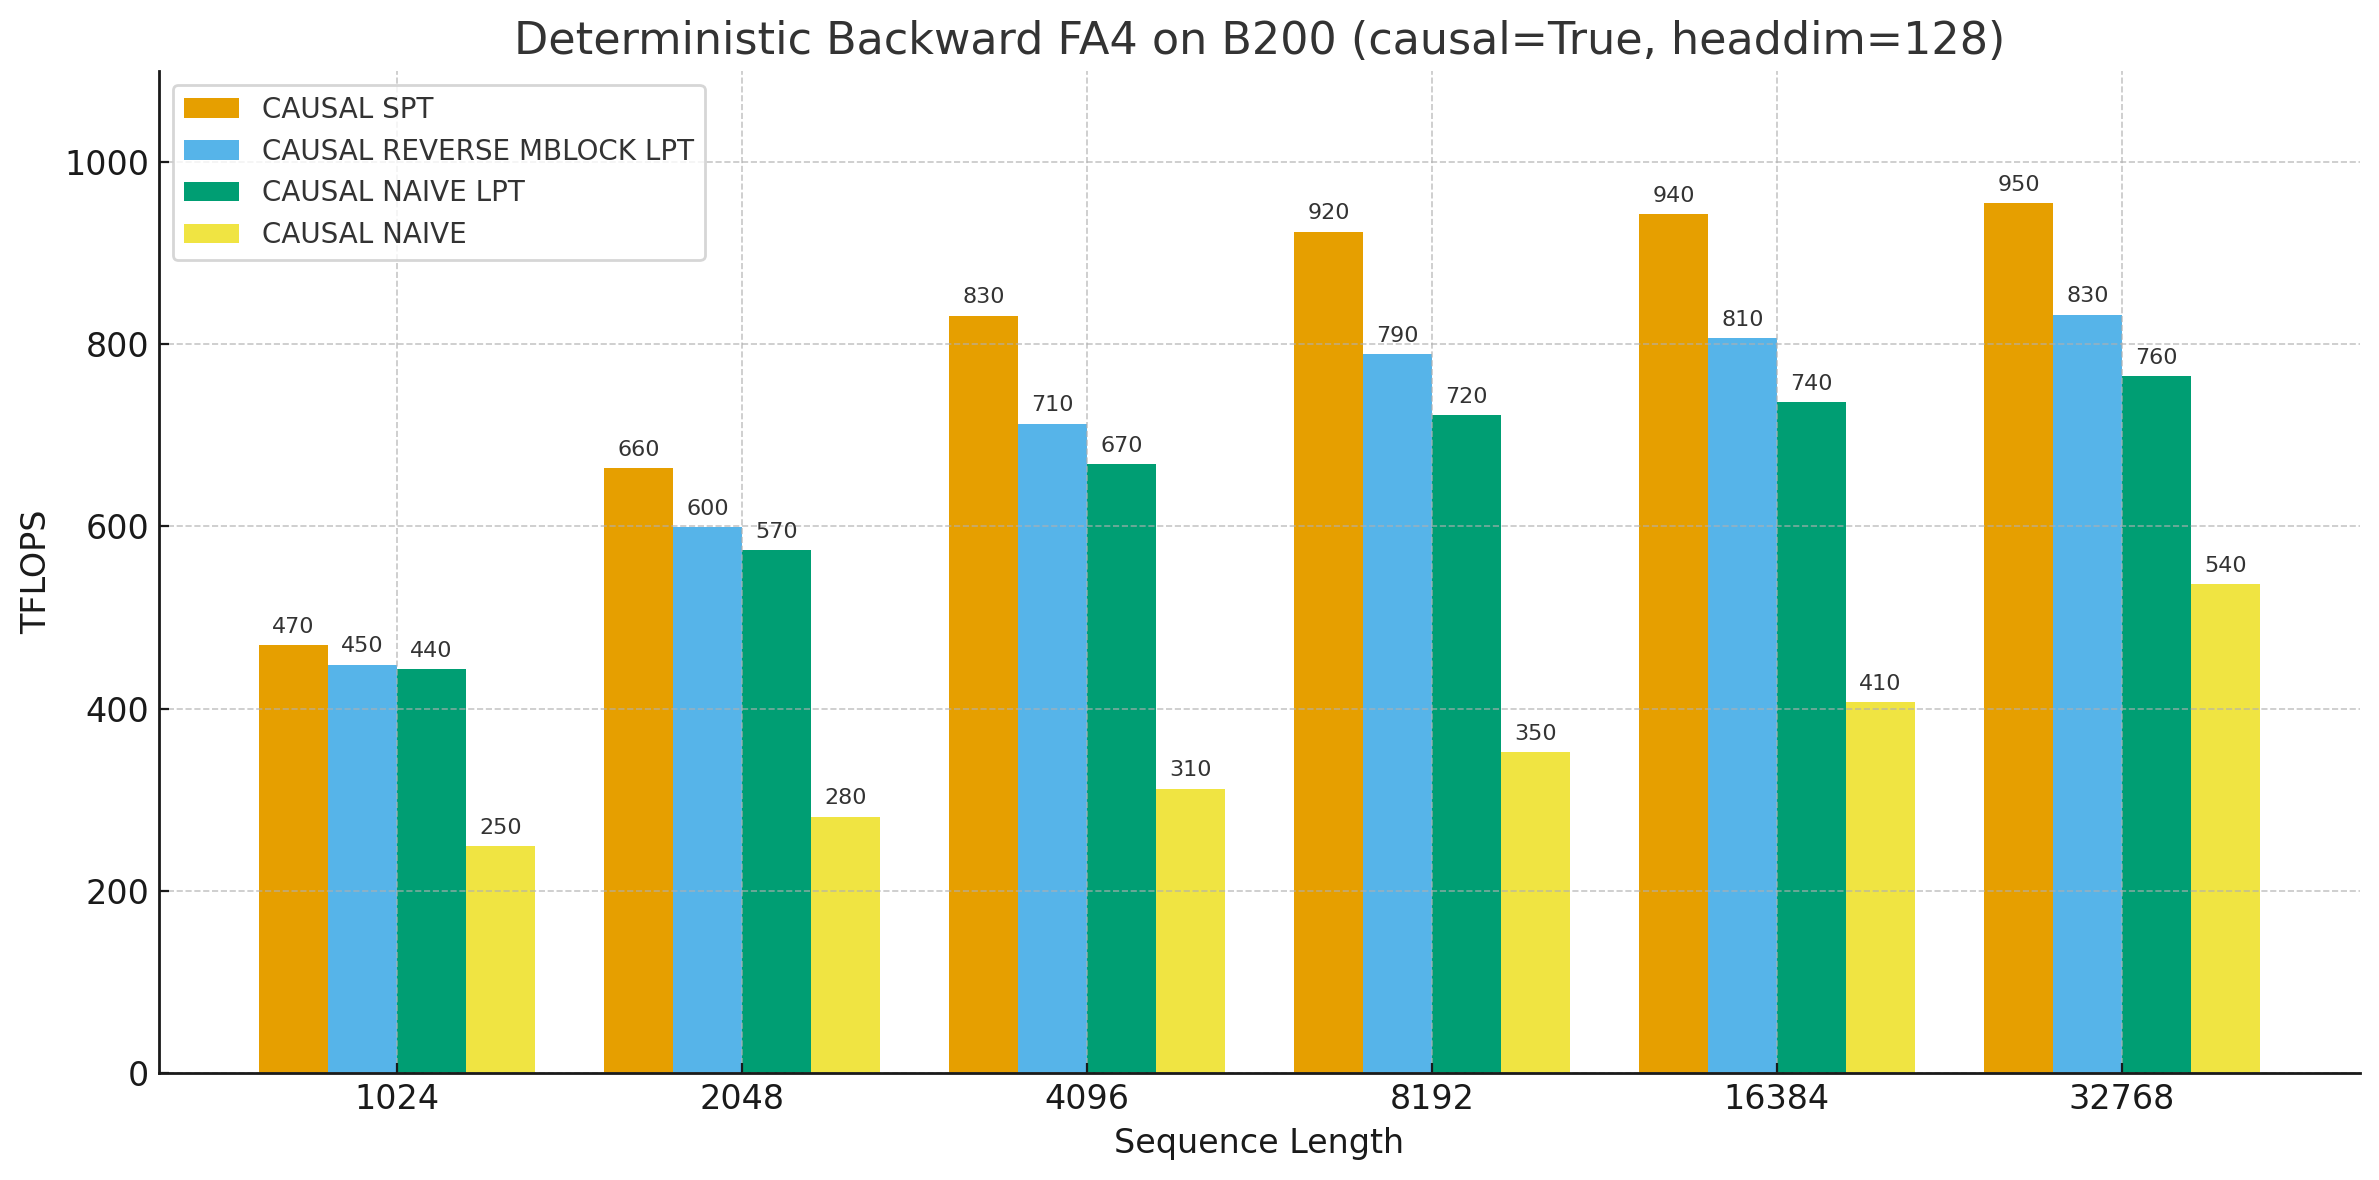
\includegraphics[width=\textwidth]{../Figures/causal_bwd_det_FA4.png}
  \end{minipage}
  \caption{B200头维度128下确定性后向传播消融实验。左：无因果注意力（带/不带批次/头重排）。右：因果注意力——SPT、逆序m块的LPT、LPT以及无批次/头重排的朴素方法。}
  \label{fig:bwd-det-ablation-non-causal}
\end{figure*}
